\documentclass{article}

\usepackage{latexsym}
\usepackage{fancyhdr}
\usepackage{algorithm}
\usepackage[noend]{algpseudocode}
\usepackage{amsmath}
\usepackage{amsthm}
\usepackage{amssymb}
\usepackage{mathtools}
\usepackage{amsthm}
\usepackage{hyperref}
\usepackage{listings}
\usepackage{dirtytalk}
\usepackage{pdfpages}
\usepackage[shortlabels]{enumitem}
\usepackage[margin=1.2in]{geometry}
\lhead{Charles Pehlivanian}
\rhead{Consecutive Partitions For Power Score Functions}
\cfoot{\thepage}
\pagestyle{fancy}

\hypersetup{colorlinks=true, urlcolor=blue}

\newtheorem{thm}{Theorem}
\newtheorem{definition}{Definition}
\newtheorem{lemma}{Lemma}
\newtheorem{sublemma}{Lemma}[lemma]

\newtheoremstyle{case}{}{}{}{}{}{:}{ }{}
\theoremstyle{case}
\newtheorem{case}{Case}

\DeclareMathOperator*{\argmax}{argmax} % thin space, limits underneath in displays
\DeclareMathOperator*{\argmin}{argmin} % thin space, limits underneath in displays
\newcommand{\stirlingii}{\genfrac{\{}{\}}{0pt}{}}

\newenvironment{example}[1]{\par\noindent\underline{Example:}\space#1}{}

\newenvironment{claim}[1]{\par\noindent\underline{Claim:}\space#1}{}
\newenvironment{claimproof}[1]{\par\noindent\underline{Proof:}\space#1}{\hfill $\blacksquare$}

\makeatletter
\def\BState{\State\hskip-\ALG@thistlm}
\makeatother

\begin{document}
\sloppy

\begin{abstract}
	This is a study consecutive partitions in the context of combinatorial optimization problems that occur in clustering, image recognition, and spatial scan statistics.
\end{abstract}

\section{Preliminaries}

Throughout $n \in \mathbb{N}$ is positive and $N = \{1, \dots, n\}$. A partition $\mathcal{P}$ of size $T$ of $N$ is specified by a set of subsets $\mathcal{P} = \{ \pi_1, \dots, \pi_T \}$, $\pi_i \subseteq N$, $i = 1, \dots, T$, such that $P_1 \cup \dots \cup P_T = \{1, \dots, n\}$, with the $P_i$'s pairwise disjoint. Each subset $\pi$ can be identified with a point $P_\pi = (\sum_{i \in \pi} x_i, \sum_{i \in \pi}y_i) \in \mathbb{R}^2$, with $P_{\emptyset} = (0,0)$ by convention.

\begin{definition}
For $\mathcal{P}$ partition of $N$, the partition polytope $\mathcal{C}$ of $\mathcal{P}$ is defined by $\mathcal{C} = convhull(\{P_\pi : \pi \in \mathcal{P}\})$. 
The constrained partition polytope of $\mathcal{P}$ is defined by $\underline{\mathcal{C}} = convhull(\{P_\pi : \pi \in \mathcal{P}$, $\pi \neq \varnothing$, $\pi \neq N\} \subseteq \mathcal{C}$. 
\end{definition}

Let $X = \left\lbrace x_1, \dots, x_n\right\rbrace$, $Y = \left\lbrace y_1, \dots, y_n\right\rbrace$ be real sequences with $y_i > 0$, for all $i$. The tuple $\left(x_i, y_i\right)$ is called a $\textit{record}$ and denoted by $R_i$. The set of records is denoted by $\mathcal{D}$. We will generally regard the sequences $X$, $Y$ as sets and study orderings on the records induced by a $\textit{priority function}$.

\begin{definition}
A priority function is a function $G\colon \mathbf{R} \times \mathbf{R}^{+} \to \mathbf{R}$ that induces an ordering on the tuples $R_i = \left(x_i, y_i\right)$. We refer to $G(x,y) = \frac{x^{\tau}}{y}$ as a power priority function, the case $\tau = 1$ being the standard priority function. The ordering induced on the sequences $X$, $Y$ induced by $G$ is denoted by $R_{(1)}, R_{(2)}, \dots R_{(n)}$, representing, in order, the highest priority record, next highest, etc. 
\end{definition}

The elements $x_i$ and $y_i$ can be thought of as contributing to a score for the record $R_{\left( i\right)}$, possibly through an excess ratio $\frac{x_i}{y_i}$, where $y_i$ represents a baseline, $x_i$ a realization, or as a normalized central moment $\frac{x_i^{\tau}}{y_i}$, weighted distance to a centroid, etc. In the area of $\textit{spatial scan}$ statistics, each record gives rise to a spatial scan statistic $\cite{article3}$ it is used by epidemiologists to detect and track ``hot spots`` or outbreaks of disease, based on diagnoses over a baseline, often assumed distributed as Poisson or Gaussian, although parametric considerations don't enter into our analysis. The notion of frequency, or realizations over a baseline motivate the properties of a score function.

\begin{definition}
A score function is a continuous function $F\colon \Omega \subseteq \mathbf{R} \times \mathbf{R}^{+} \to \mathbf{R}$ that is increasing in $x$ and decreasing in $y$. If F is of the form $F(x,y) = \frac{x^\gamma}{y}$ for some $\gamma > 0$, then F is a power score function. 
\end{definition}

Several additional properties have been associated with score functions, namely quasi-convexity, marginal convexity in the individual variables, or a marginal contribution constraint $\frac{x}{y} \frac{\partial F}{\partial x} + \frac{\partial F}{\partial y} \geq 0$ related to submodularity. In particular we do not assume smoothness beyond continuity, nor convexity, unless explicitly stated.

We extend the functions $F$, $G$ to subsets of $X_i \in X$, $Y_i \in Y$ by defining $F(X_i, Y_i) = F(\sum_{x_i \in X_i} x_i, \sum_{y_i \in Y_i} y_i)$. We also use the notation $X_1 = \sum_{x_i \in X_i}x_i$, $Y_1 = \sum_{y_i \in Y_i}y_i$, etc. So any score function can be regarded as a function $F \colon 2^X \to \mathbf{R}$.

\vspace{4pt}

The notion of consecutive subset needs to be refined in order to distinguish strongly consecutive partitions from weakly consecutive ones. 

\begin{definition}
A subset $S \subseteq N$ is consecutive if it is of the form $\left\lbrace j, j+1, \dots k\right\rbrace$, for $1 \leq j \leq k \leq n$. A consecutive subset $\pi \subseteq N$ is non-splitting if both $\pi$, $N  \backslash \pi$ are consecutive. Otherwise, it is splitting. Designate
\begin{align*}
C &= C_N = \{ \pi \subseteq N : \pi \textrm{ is consecutive} \}\\
U &= U_N = \{ \pi \subseteq N : \pi \textrm{ is consecutive, non-splitting}\} \\
S &= S_N = C \backslash U = \{ \pi \subseteq N : \pi \textrm{ is consecutive, splitting} \}
\end{align*}
\end{definition}

A special case of a splitting subset occurs when one of $S$, $N$ is a singleton, which we call a singleton splitting pair. It is easy to see that $| U_N | = 2n - 1$, $| S_N | = \frac{(n-1)(n-2)}{2}$, with $|C_N| = |U_N| + |S_N| = \frac{n(n+1)}{2}$. Therefore, a search over consecutive non-splitting portfolios can be performed in linear time. If a singleton subset $\{ i \} \subseteq N$ is splitting (i.e.\ if $1 < i < n$), then we call the pair $\{ \{i\}, N\backslash_{\{i\}} \}$ a singleton splitting pair.


Let $\mathcal{P}$ be a partition of the set $N = \{1, \dots, n\}$. We are interested in solutions to the optimization problem
\begin{align} \label{eq0}
\mathcal{P} = \max_{\mathcal{P}, \vert \mathcal{P} \vert = T} {\sum\limits_{j=1}^{T}F\left( X_j, Y_j\right)}
\end{align}
which for a power score function becomes
\begin{align} \label{eq1}
\mathcal{P} = \max_{\mathcal{P}, \vert \mathcal{P} \vert = T}\sum_{j=1}^{T}\frac{(\sum_{R_i \in P_j}x_i)^\gamma}{\sum_{R_i \in P_j}y_i}
\end{align}

For $\gamma \geq 0$. For example, given a set of quadratic polynomials $f_i(x) = \frac{1}{2}h_ix^2 + g_ix + c_i$, with $h_i >0$ for all $i$, the $x$ values of the vertices are given by $\frac{-g_i}{h_i}$, with minimum values $\frac{-g_i^2}{2h_i}$. The standard priorty function puts an ordering on the vertices sequences $\left\lbrace g_i\right\rbrace$, $\left\lbrace h_i  \right\rbrace$ which is equivalent to projection onto the x-coordinate of the vertex $\left(\frac{-g_i}{h_i},\frac{-g_i^2}{2h_i}\right)$. For $T = 1$, we can easily minimize the sum $\sum_{i=1}^{n} f_i(x)$. For $T >= 2$ the optimization in $\ref{eq1}$ with $\gamma = 2$ finds the $x$-values $\left\lbrace x_1, \dots x_T\right\rbrace$ and the partition that minimize the sum $\sum_{j=1}^T \sum_{i \in P_j} f_i\left( x_j\right)$. This can also be viewed in the context of gradient boosting, in which the maximal partition represents optimal leaf values for a classifier that can take at most $T$ values.

It is well-known that the optimization in $\ref{eq1}$ is NP-complete, for general score functions, even for power score functions. It will be necessary to constrain the optimization in \ref{eq1} and restrict our attention to subsets of the set of all partitions of $n$, itself a large set.

\begin{definition}
A partition $\mathcal{P}$ such that each $P_i$ is an ordered subsequence of $\left\lbrace 1, \dots N\right\rbrace$, so that $P_i = \{R_{(j)}, \dots, R_{(j+l_i)}\}$, for some $j$, is called a consecutive partition. If every subset of a consecutive partition is nonempty, then it is strongly consecutive. 
If in addition the (strongly) partition satisfies
\[
\mathcal{P} = \argmax_{\mathcal{P}, \vert \mathcal{P} \vert = T}\sum_{j=1}^{T}F\left( X_j, Y_j \right)
\]
then $\mathcal{P}$ is a maximal (strongly) consecutive partition for the power score function $F(x,y) = \frac{x^\gamma}{y}$. A maximal partition that contains only consecutive non-splitting and at least one splitting subset is called a maximal splitting partition.
\end{definition}

The set of partitions is greatly reduced by the requirement that $\mathcal{P}$ be ordered. The set of all partitions of $n$ is the Bell number of order $T$, exponentially increasing with $n$ for any $T > 1$. The set of all size $T$ partitions is a Stirling number of the second kind $\stirlingii{n}{T}$. The $n$th Bell number $B_n$ is given by the identity
\[B_n = \sum_{k=0}^{n} \binom{n}{k} B_k\]
The Stirling numbers follow the recursion
\[\stirlingii{n+1}{k} = k\stirlingii{n}{k} + \stirlingii{n}{k-1}\]
and have asymptotic growth rate 
\[\stirlingii{n}{k} \sim \frac{k^n}{k!}\]
So, for example, for $\left(n,T\right) = \left(20, 10\right)$, we have $B_n \approx 5.9e12$, $\mathcal{O} = 92378$, while for $\left(n,T\right) = \left(30, 10\right)$, we have $B_n \approx 1.73e22$, $\mathcal{O} = 10,015,005$.

If the object is to optimize \eqref{eq0} over partitions of strict size $T$, these results are not of much help. There is no guarantee that a strictly maximal partition exists, and the search space cannot be reduced. If the object is to find a consecutive partition of strict size $S \le T$, we are in worse shape; all partitions of size $T$ must be examined. If the optimizing partition is consecutive, we're done. Otherwise, we must repeat the process for size $T$ - 1. 

\vspace{4pt}

It will be shown that, for the class $\mathcal{F}_{\gamma} \times \mathcal{G}_{\tau}$, the guaranteed existence of a strongly consecutive maximal partition is rare. \ref{thm0}. An improved, efficient determination of the optimal consecutive partition, weak or not, is described, allowing for a search over a smaller subset and a worst-case $O(N^2)$ algorithm. Applications to $<\dots>$ are given in Section 3.


It is known (see $\cite{article1}$, $\cite{article2}$) that if $F$ is convex in all of its arguments, and 
$y \geq 0$ (by convention $\frac{x_i}{0} = \infty$), that a weakly consecutive partition exists for the standard priority function. Unfortunately the weakly consecutive partitions can collapse spectacularly to the degenerate case $T=1$ without additional assumptions.

\begin{example}
Let $X = \left\lbrace 8, 2, 9\right\rbrace$, $Y = \left\lbrace  8, 1, 3\right\rbrace$, $G$ the standard priority function and $F$ the power score function with $\gamma = 4$. It is clear that $F$ is argument-wise convex. There are 3 partitions of the set $N = \left\lbrace 1,2,3 \right\rbrace$ and direct evaluation gives
\begin{verbatim}
      PARTITION: [[1, 2], [3]]
          SUBSET: [1, 2] SUBSET SCORE: 1111.1111
          SUBSET: [3] SUBSET SCORE: 2187.0
          PARTITION SCORE: 3298.1111
      PARTITION: [[1], [2, 3]]
          SUBSET: [1] SUBSET_SCORE: 512.0
          SUBSET: [2, 3] SUBSET SCORE: 3660.25
          PARTITION SCORE: 4172.25
      PARTITION: [[1, 3], [2]]
          SUBSET: [1, 3] SUBSET SCORE: 7592.8182
          SUBSET: [2] SUBSET SCORE: 16.0
          PARTITION SCORE: 7608.8182
      MAX PARTITION SCORE: 7608.8182, MAX_PARTITION: [[1, 3], [2]]
\end{verbatim}
In this case no strongly consecutive partition of size 2 exists as the optimal partition is nonconsecutive. A weakly consecutive partition of size $T = 1$ exists consisiting of the trivial partition of $N$ with dominating score
\begin{verbatim}
      PARTITION: [[1, 2, 3]]
          SUBSET: [1, 2, 3] SUBSET SCORE: 10860.0833
          PARTITION SCORE: 10860.0833
      MAX PARTITION SCORE: 10860.0833, MAX_PARTITION: [[0, 1, 2]].
\end{verbatim}  
\end{example}

\begin{example}
Let 
\begin{align*}
X & = \left\lbrace 0.992819 0.04904 0.622353 0.464107 0.608956 0.984192 \right\rbrace \\
Y & = \left\lbrace 0.935323 0.02541 0.279373 0.205452 0.24599 0.315633 \right\rbrace,
\end{align*}
$G$ the standard priority and $\gamma = 4$. $\frac{X}{Y} = \left\lbrace 1.0614718 1.9299488 2.2276777 2.2589559 2.4755315 3.118153 \right\rbrace$. $F$ is convex in each of its arguments, but the only maximal consecutive partition of size $T = 5$ is the trival size-1 partition. We have

\begin{verbatim}
    Maximal 5-partition
    PARTITION: [ 0 5 ][ 1 ][ 2 ][ 3 ][ 4 ]
    SUM OF SCORES: 13.5342629367

    Maximal 4-partition
    PARTITION: [ 0 4 5 ][ 1 ][ 2 ][ 3 ]
    SUM OF SCORES: 30.6365105858

    Maximal 3-partition
    PARTITION: [ 0 2 4 5 ][ 1 ][ 3 ]
    SUM OF SCORES: 59.8732051128

    Maximal 2-partition
    PARTITION: [ 0 2 3 4 5 ][ 1 ]
    SUM OF SCORES: 91.7825870559

    Maximal 1-partition
    PARTITION: [ 0 1 2 3 4 5 ]
    SUM OF SCORES: 95.5586821397
\end{verbatim}
In fact the trivial partition is the optimal partition of size $T \leq 5$, and there are no strongly consecutive maximal partitions for any $T \in \left\lbrace 1, 2, 3, 4, 5\right\rbrace$.

\end{example}
In fact for any pair $\left( N, T\right)$ a maximally-degenerate collapsing exists for most score functions. This degeneracy is alluded to in the proof of the main result in $\cite{article1}$, $\cite{article2}$, although it is more prevalent than the authors indicate. In particular, any search over the consecutive partitions of size $T$ at the top level is incomplete; it may be the case that the optimal partition is weakly consecutive, in which case, the only way to determine this is to search over $\textit{all}$ partitions, consecutive or otherwise, at top level, to determine whether indeed the the optimal consecutive partition is truly of size $T$. If not, if a nonconsecutive partition exists at size $T$ that is optimal, one must do the entire search at level $T-1$ again. There is no efficiency gain if one knows in advance only that the optimal partition is weakly consecutive. 

\section{Main Results}
{\parindent0pt % disables indentation for all the text between { and }
We now state our main results.
}% restore indentation
\newtheorem{prop} \label{thm0}
\textbf{Proposition} Let $\mathcal{P}$ be a partition of $N$, and let $\mathcal{E} = \mathcal{E}_\mathcal{C} = \{$ extreme points of $\mathcal{C}$ \}, $\underline{\mathcal{E}} = \mathcal{E}_{\underline{\mathcal{C}}} = \{$ extreme points for $\underline{\mathcal{C}}$ \}. Then
\begin{enumerate}[(i)]
	\item $\mathcal{E} = \{P_\pi$ : $\pi \in U_N$\}
	\item $\underline{\mathcal{E}} \supseteq \{P_\pi$ : $\pi \in U_N\setminus\left\lbrace p_{\emptyset}, p_N \right\rbrace$\}, with the possible addition of singleton splitting pairs.
\end{enumerate}
In particular $\underline{\mathcal{E}}$ may contain splitting elements while $\mathcal{E}$ never does.

\vspace{6pt} 


\begin{thm} \label{thm1}
Let the dataset $\mathcal{D} = \{ \mathbf{R}_1, \ldots, \mathbf{R}_n \}$ be ordered with priority function $G(\mathbf{R}_i) = G(x_i,y_i) =  \frac{x_i^\tau}{y_i}$, and equipped with the score function $F(\mathbf{R}_i) = f(x_i,y_i) = \frac{x_i^\gamma}{y_i}$. $F_1x \times T \in \mathbb{N},$ $T < N$. Then there is a strongly maximally ordered partition of non-splitting subsets of size $T$ iff $(\gamma, \tau) = (2,1)$.
\end{thm}

\begin{thm} \label{thm2}
$\mathcal{D}$, $F$, $G$ as above. If $F$ is quasiconvex, then there is either a strongly consecutive maximal non-splitting partition, or a consecutive singleton splitting maximal partition.
\end{thm}

The notion of 

The brute-force optimization in $\ref{eq1}$ has cost that grows exponentially with $n$. A constrained optimization over the set of all size $T$ ordered partitions has cost that grows as $\binom{n-1}{T-1}$, i.e., as a polynomail of degree $T-1$. In particular, the $T = 2$ problem grows linearly in $n$. There is an improvement that can be made to this approach.

Consider a graph $\mathcal{G} = \left( V, E\right)$ with vertices denoted by $\left( i, j\right)$, for $i \in \left\lbrace 1, \dots, n\right\rbrace$, $j \in \left\lbrace 1, \dots, T\right\rbrace$. Add a source node $\left( 1, 1\right)$ and a terminal sink node labeled $\left( n+1, T+1\right)$, Add directed edges from node $\left( i,k \right)$ to $\left( i, k+1\right)$, for each $i < j$, with edge cost $\frac{-\left(\sum_{r=i}^{j-1} x_r\right)^2}{\sum_{r=i}^{j-1} y_r}$. The interpretation is that a path from node $\left( i, j\right)$ to $\left( k, j+1\right)$ represents choice of the subset $\left\lbrace i, \dots, k\right\rbrace$ as the $i^{th}$ subset in the candidate partition. One can then solve for the shortest path by finding a shortest path by the Bellman-Ford algorithm. 


% 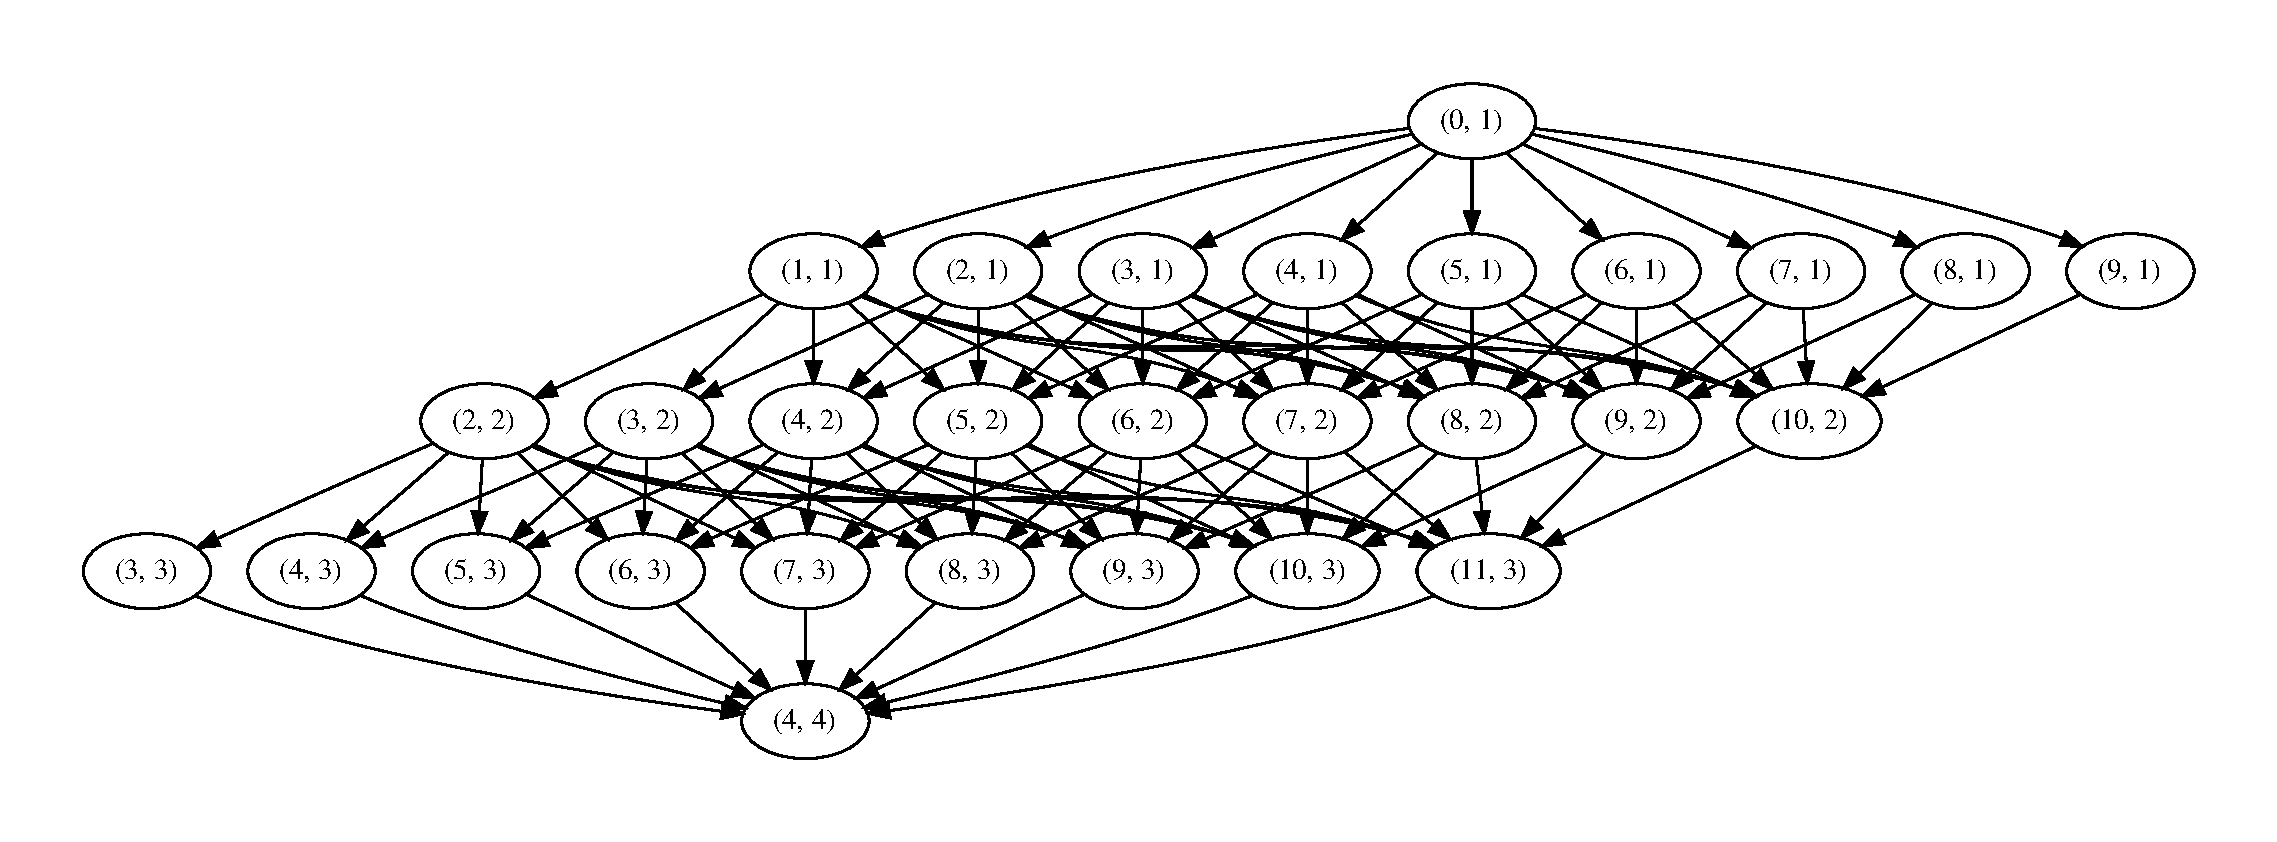
\includepdf[pages=-]{12_4_unlabeled.pdf}
\begin{figure}
  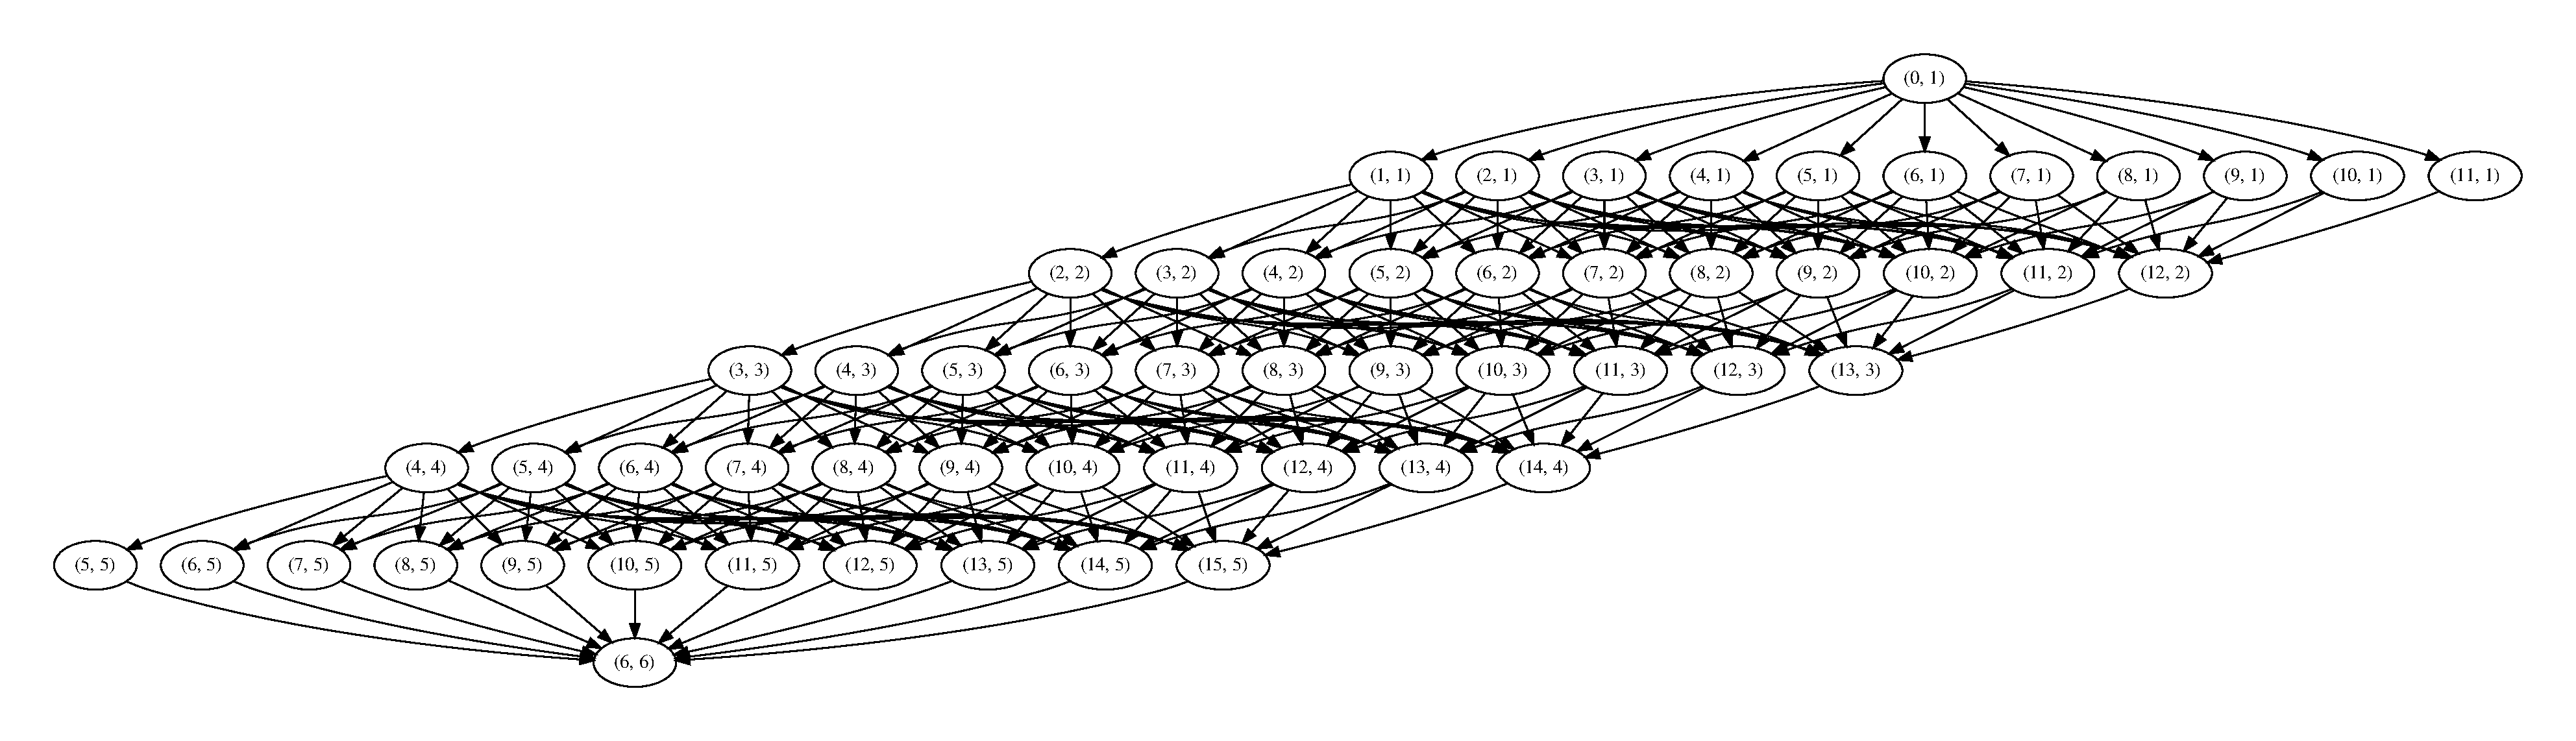
\includegraphics[scale=.22]{16_6_unlabeled.pdf}
  \caption{Graph connectivity, (N, T) = (16, 6)}  
\end{figure}

\vspace{16pt}
\begin{figure}
  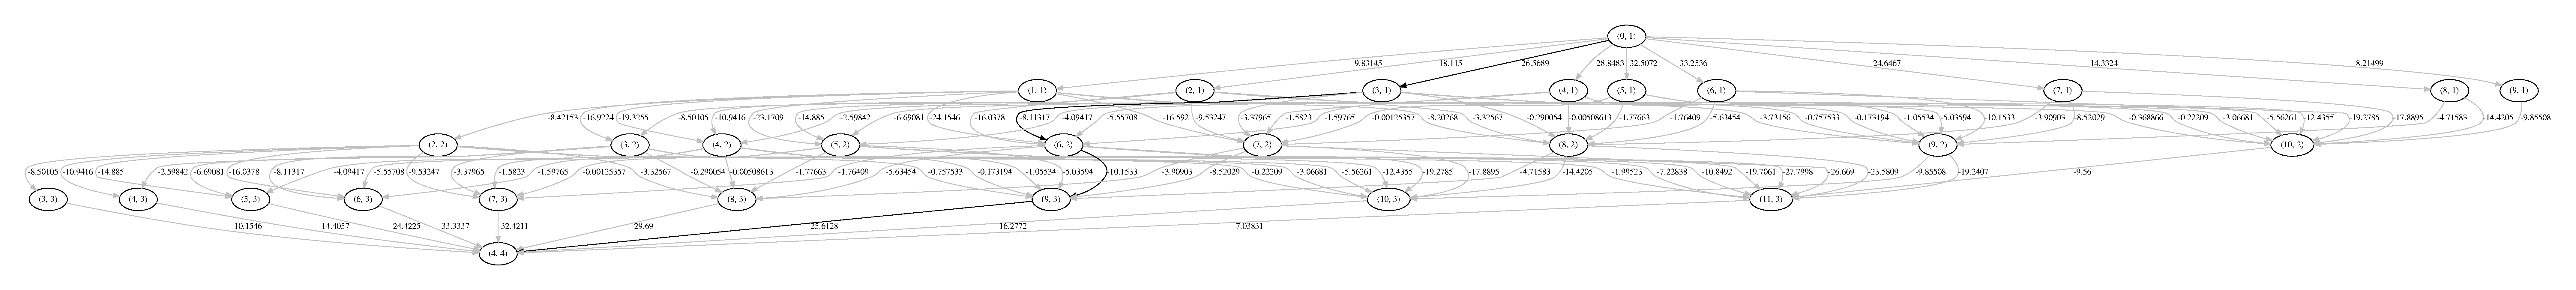
\includegraphics[scale=.11]{12_4_labeled.pdf}
  \caption{Labeled (N, T) = (12, 4) case displaying optimal path SOURCE -- (0, 3) -- (3, 6) -- (6, 9) -- (9, 12) --  SINK corresponding to ordered partition [[0 1 2 ], [3 4 5 ], [6 7 8 ], [9 10 11 ]]}
\end{figure}

For the graph $\mathcal{G} = \left( V, E\right)$, we have 
\begin{align*}
\vert V \vert & = \left( T-1\right)\left(N-T-1\right) + 2 \\
\vert E \vert & = 2\left( N-T+1\right) + \left( T-1\right)\sum_{i=1}^{N-T+1} i = 2\left( N-T+1\right) + \frac{T-1}{2}\left( N-T+1\right)\left( N-T+2\right)
\end{align*}

The Bellman-Ford algorithm requires $\mathcal{O}\left( V\cdot E\right)$ operations, which for $N >> T$ is $\mathcal{O}\left( TN^2\right)$. A naive search of all ordered partitions requires $\binom{n-1}{T-1}$ operations, a polynomial of order $T-1$ in $N$. We have effectively reduced large cases to be no worse than quadratic in N. The time savings is at the expense of memory footprint; all partial sums of the form $\frac{-\left(\sum_{r=i}^{j-1} x_r\right)^2}{\sum_{r=i}^{j-1} y_r}$ must be stored (although sequential calculation cost is still $\mathcal{O}\left( N\right)$). This may be the most significant feature of this approach - all partial sums are cached on a computation tree that is easily traversed. For example, for a sample size of 10,000 points, with T = 100, there are approximately 4.8530e9 edges, with a storage cost of approximately 19.4119 Gb. Running times are quite fast, however, and we are currently exploring a distributed version of the algorithm.

\cleardoublepage
\appendix
\section{Appendix}
We present here an alternative proof of Theorem 1 which is elementary and direct.

\vspace{6pt}

$\textit{Proof of Theorem 1}$
For sufficiency, let $\gamma = 2$, and suppose the partition $\mathcal{P} = \left\lbrace P_1, \dots, P_T\right\rbrace$ is the argmax solution to \ref{eq1}. Let $R_1 = (X_1, Y_1)$ be the set of records in $\mathcal{P}$ that contains the maximal element $R_{(1)}$ of $\mathcal{D}$, and define $R_1^{in} = \argmin_{R_j \in X_1} G(x_i, y_i)$, $R_1^{out} = \argmax_{R_j \not\in X_1} G(x_i, y_i)$. Note that $X_1$ is an ordered subset if and only if $R_1^{in} <= R_1^{out}$, so that there are no "holes" in $X_1$. This is not true if $X_1$ does not contain the maximal element. This can be made precise by defining $I_1^{in} = j \text{ such that} R_{(j)} = R_1^{in}$, $I_1^{out} = j \text{ such that} R_{(j)} = R_1^{out}$, and $D_1 = I_1^{in} - I_1^{out}$. It is then the case that $D_1 \geq 1$, and $X_1$ is ordered if and only iff $D_1 < 0$.

Set $D = D_1$ and assume $D_1 \geq 0$. We describe an iterative procedure that swaps elements between $X_1$ and the remaining subsets, such that each step does not decrease the overall score of the partition, and decreases the value of $D$ by at least 1. In this way the procedure can be stopped when $X_1$ is ordered. We can then remove $X_1$ from the partition, regarding the remaining subsets as a partition of $\left\lbrace 1, \dots N-\vert X_1 \vert\right\rbrace$, and apply the same procedure to the remaining subset containing the maximal element. The process terminates with a maximal ordered partition.

\begin{algorithm}
\caption{Ordering Algorithm: Single Subset}
\begin{algorithmic}[1]
\State $\textit{Select } X_1 \textit{ containing maximal element of } \mathcal{D}$
\State $\left( \alpha , \beta \right) \gets R_1^{in}, \left( a,b \right) \gets R_1^{out}$
\State $D \gets I_1^{in} - I_1^{out}$
\While{$D \geq 0$}
\If{$X_1, X_2 \geq 0$}
\State $X_1^\prime \gets X_1\setminus \left\lbrace x_1^{in}\right\rbrace$, $Y_1^{\prime} \gets X_1\setminus \left\lbrace y_1^{in}\right\rbrace$
\State $X_2^{\prime} \gets X_2\cup \left\lbrace x_1^{in}\right\rbrace$, $Y_2^{\prime} \gets X_2\cup \left\lbrace y_1^{in}\right\rbrace$
\EndIf
\If{$X_1, X_2 \leq 0$}
\State $X_1^{\prime\prime} \gets X_1\cup \left\lbrace x_1^{out}\right\rbrace$, $Y_1^{\prime\prime} \gets X_1\cup \left\lbrace y_1^{out}\right\rbrace$
\State $X_2^{\prime\prime} \gets X_2\setminus \left\lbrace x_1^{out}\right\rbrace$, $Y_2^{\prime\prime} \gets X_2\setminus \left\lbrace y_1^{out}\right\rbrace$
\EndIf
\If{$X_1 \leq 0, X_2 \geq 0 \textit{ or } r X_1 \geq 0, X_2 \leq 0$}
\State $\left\lbrace X_1, Y_1, X_2, Y_2 \right\rbrace \gets \textit{one of } \left\lbrace X_1^{\prime}, Y_1^{\prime}, X_2^{\prime}, Y_2^{\prime}\right\rbrace, \left\lbrace X_1^{\prime\prime}, Y_1^{\prime\prime}, X_2^{\prime\prime}, Y_2^{\prime\prime}\right(\rbrace$
\EndIf
\State {$D \gets I_1^{in} - I_1^{out}$}
\EndWhile
\end{algorithmic}
\end{algorithm}

% \begin{algorithm}
% \caption{Ordering Algorithm}\label{Algorithm}
% \begin{algorithmic}[1]
% \Procedure{MyProcedure}{}
% \State $\textit{stringlen} \gets \text{length of }\textit{string}$
% \State $i \gets \textit{patlen}$
% \BState \emph{top}:
% \If {$i > \textit{stringlen}$} \Return false
% \EndIf
% \State $j \gets \textit{patlen}$
% \BState \emph{loop}:
% \If {$\textit{string}(i) = \textit{path}(j)$}
% \State $j \gets j-1$.
% \State $i \gets i-1$.
% \State \textbf{goto} \emph{loop}.
% \State \textbf{close};
% \EndIf
% \State $i \gets i+\max(\textit{delta}_1(\textit{string}(i)),\textit{delta}_2(j))$.
% \State \textbf{goto} \emph{top}.
% \EndProcedure
% \end{algorithmic}
% \end{algorithm}


 Without loss of generality, assume $R_1^{out} \in X_2$. We will assume that $G(x_1^{in}, y_1^{in}) < G(x_1^{out}, y_1^{out})$, and show that we can obtain an improvement in the sum $F(X_1, Y_1) + F(X_2, Y_2)$ by exchanging elements of $X_1$, $X_2$. In this way the elements of the subset $X_1$ are sucessively swapped out until it is ordered. Since $X_1$ is the partition with maximal element, we can remove it from consideration, and find the maximal remaining element, and apply the same procedure. In this way we obtain a partition all of whose subsets are ordered.

Assume the tuples $R_1^{in}$, $R_1^{out}$ are composed of $R_1^{in} = \left(x_1^{in}, y_1^{in}\right), R_1^{out} = \left(x_1^{out}, y_1^{out}\right)$.

Define
\begin{align*}
X^\prime\left( \lambda \right) & = \lambda \left( X_1 - x_1^{in}\right) + \left( 1 - \lambda\right) \left( X_1^\prime + x_1^{out}\right) \\
Y^\prime\left( \lambda \right) & = \lambda \left( Y_1 - y_1^{in}\right) + \left( 1 - \lambda\right) \left( Y_1^\prime + y_1^{out}\right)
\end{align*}

for $\lambda \in \left[ 0,1\right]$. For $\lambda_{*} = \frac{y_1^{out}}{y_1^{in} + y_1^{out}}$, we have $Y^\prime\left( \lambda_{*}\right) = Y_1$, and 
\[X^\prime\left( \lambda_{*}\right) = X_1 + \frac{y_1^{in}x_1^{out}-y_1^{out}x_1^{in}}{y_1^{in} + y_1^{out}}\]

Since $G(x_1^{in}, y_1^{in}) < G(x_1^{out}, y_1^{out})$, $\frac{y_1^{in}x_1^{out}-y_1^{out}x_1^{in}}{y_1^{in} + y_1^{out}} > 0$ and $X^\prime\left( \lambda_{*}\right) > 0$. We therefore have 
\begin{align} \label{eq2}
F(X_1, Y_1) \leq F(X^\prime\left( \lambda \right), Y_1) \leq \lambda\left( F(X_1-x_1^{in},Y_1-y_1^{in})\right) + \left( 1 + \lambda\right)\left( F(X_1+x_1^{out},Y_1+y_1^{out})\right)
\end{align}
where the second inequality is from the quasiconvexity of $F$ for $\gamma = 2$. From \ref{eq2} it follows that 
\begin{align} \label{eq3}
F(X_1, Y_1) \leq \max{\left(F(X_1-x_1^{in},Y_1-y_1^{in}), F(X_1+x_1^{out},Y_1+y_1^{out})\right)}
\end{align}

To get a similar result for the sets $X_2$, $Y_2$, define the transformed sequences $\bar{X} = \left\lbrace -x_1, \dots, -x_n\right\rbrace$, $\bar{Y} = \left\lbrace y_1, \dots, y_n\right\rbrace$. The sets $\bar{X_1}, \bar{X_2}, \bar{Y_1}, \bar{Y_2}$ are similarly defined, and we can define $\bar{R_2}^{in} = \argmin_{\bar{R_j} \in \bar{X_2}} G(\bar{x_i}, \bar{y_i})$, $\bar{R_1}^{out} = \argmax_{\bar{R_j} \not\in \bar{X_1}} G(\bar{x_i}, \bar{y_i})$. Assuming the correspondence between record and underlying sequences $\bar{R}_i = \left(\bar{x_i}, \bar{y_i}\right)$, we then have $x_1^{in} = -\bar{x}_2^{out}$, $y_1^{in} = \bar{y_2}^{out}$, and $x_1^{out} = -\bar{x}_2^{in}$, $y_1^{out} = \bar{y_2}^{in}$. 

Define
\begin{align*}
\bar{X}^\prime\left( \lambda \right) & = \lambda \left( \bar{X_2} - \bar{x_2}^{in}\right) + \left( 1 - \lambda\right) \left( \bar{X_2} + \bar{x_2}^{out}\right) \\
\bar{Y}^\prime\left( \lambda \right) & = \lambda \left( \bar{Y_2} - \bar{y_2}^{in}\right) + \left( 1 - \lambda\right) \left( \bar{Y_2} + \bar{y_2}^{out}\right)
\end{align*}

for $\lambda \in \left[ 0,1\right]$. For $\bar{\lambda}_{*} = \frac{\bar{y_2}^{out}}{\bar{y_2}^{in} + \bar{y_2}^{out}}$, we have $\bar{Y}^\prime\left( \bar{\lambda}_{*}\right) = \bar{Y_1}$, and 
\[\bar{X}^\prime\left( \bar{\lambda}_{*}\right) = \bar{X_2} + \frac{\bar{y_2}^{in}\bar{x_2}^{out}-\bar{y_2}^{out}\bar{x_2}^{in}}{\bar{y_2}^{in} + \bar{y_2}^{out}}\]
By similar arguments, and since $\bar{y_2}^{in}\bar{x_2}^{out}-\bar{y_2}^{out}\bar{x_2}^{in} = x_1^{out}y_1^{in} - x_1^{in}y_1^{out} \geq 0$, 
\begin{align*}
F(X_2, Y_2) = F(\bar{X_2}, \bar{Y_2}) & \leq \max{\left(F(\bar{X_2}-\bar{x_2}^{in},\bar{Y_2}-\bar{y_2}^{in}), F(\bar{X_2}+\bar{x_2}^{out},\bar{Y_2}+\bar{y_2}^{out})\right)} \\
& = \max{\left(F(\bar{X_2}-\bar{x_2}^{in},Y_2-y_1^{our}), F(\bar{X_2}+\bar{x_2}^{out},\bar{Y_2}+y_2^{out})\right)} \\
& = \max{\left(F(\bar{X_2} +x_1^{out},Y_2-y_1^{out}), F(\bar{X_2}-x_1^{in},Y_2+y_2^{out})\right)} \\
& = \max{\left(F(X_2 -x_1^{out},Y_2-y_1^{out}), F(X_2+x_1^{in},Y_2+y_2^{out})\right)}
\end{align*}

So
\begin{align} \label{eq4}
F(X_2, Y_2) \leq \max{\left(F(X_2-x_1^{out},Y_2-y_1^{out}), F(X_2+x_1^{in},Y_2+y_1^{in})\right)}
\end{align}

If we form the table
\[
\begin{pmatrix}
&F(X_1 - x_1^{in}, Y_1 - y_1^{in}) & F(X_2 + x_1^{in}, Y_2 + y_1^{in}) \\
&F(X_1 + x_1^{out}, Y_1 + y_1^{out}) & F(X_2 - x_1^{out}, Y_2 - y_1^{out})
\end{pmatrix} = \begin{pmatrix}
&A_{11} & A_{12} \\
&A_{21} & A_{22}
\end{pmatrix}
\]
then the results in \ref{eq2}, \ref{eq4} imply that $F(X_1, Y_1) \leq \max{\left(A_{11}, A_{21}\right)}$ and $F(X_2, Y_2) \leq \max{\left(A_{12}, A_{22}\right)}$. What we would like to show is that $F(X_1, Y_1) + F(X_2, Y_2) \leq \max{\left(A_{11}, A_{12}\right)}$ or $F(X_1, Y_1) + F(X_2, Y_2) \leq \max{\left(A_{21}, A_{22}\right)}$, as those operations represent a swap of records between the two sets $X_1$, $X_2$. To this end assume that the maximum values down columns occur in different rows, e.g. $\max{\left(A_{11}, A_{21}\right)} = A_{11}$, $\max{\left(A_{12}, A_{22}\right)} = A_{22}$. The case for which the maximums occur on the opposite diagonal is handled similarly. We can then assume that 
\begin{align}
& F(X_1 - x_1^{in}, Y_1 - y_1^{in}) - F(X_1, Y_1) \geq 0 \\
& F(X_2 - x_1^{out}, Y_2 - y_1^{out}) - F(X_2, Y_2) \geq 0 \\
& F(X_1 + x_1^{out}, Y_1 + y_1^{out}) - F(X_1, Y_1) \leq 0 \\
& F(X_2 + x_1^{in}, Y_2 + y_1^{in}) - F(X_2, Y_2) \leq 0
\end{align}

Expand 
\[
F(X - \alpha, Y - \beta) - F(X, Y) = \frac{\beta X^2 - 2\alpha XY + \alpha^2 Y}{Y\left( Y-\beta\right)}
\]
and write
\begin{align*}
F(X_1 - x_1^{in}, Y_1 - y_1^{in}) + F(X_2 + x_1^{in}, Y_2 + y_1^{in}) - \left( F(X_1, Y_1) + F(X_2, Y_2)\right) = \\
\left( F(X_1 - x_1^{in}, Y_1 - y_1^{in}) - F(X_1 - x_1^{in}, Y_1)\right) + \left( F(X_1 - x_1^{in}, Y_1) - F(X_1 , Y_1)\right) + \\
\left( F(X_2 + x_1^{in}, Y_2 + y_1^{in}) - F(X_2 + x_1^{in}, Y_2)\right) + \left( F(X_2 + x_1^{in}, Y_2) - F(X_2, Y_2)\right)
\end{align*}

and
\begin{align*}
F(X_1 + x_1^{out}, Y_1 + y_1^{out}) + F(X_2 - x_1^{out}, Y_2 - y_1^{out}) - \left( F(X_1, Y_1) + F(X_2, Y_2)\right) = \\
\left( F(X_1 + x_1^{out}, Y_1 + y_1^{out}) - F(X_1 + x_1^{out}, Y_1)\right) + \left( F(X_1 + x_1^{out}, Y_1) - F(X_1 , Y_1)\right) + \\
\left( F(X_2 - x_1^{out}, Y_2 - y_1^{out}) - F(X_2 - x_1^{out}, Y_2)\right) + \left( F(X_2 - x_1^{out}, Y_2) - F(X_2, Y_2)\right)
\end{align*}

For ease of notation designate $\alpha = x_1^{in}$, $\beta = y_1^{in}$, $a = x_1^{out}$, $b = y_1^{out}$.

The summands for the top equation can then be written
\begin{align*}
s_1 & = \frac{\left(X_1 - \alpha\right)^2\beta}{Y_1\left( Y_1 - \beta\right)} \\
s_2 & = \frac{\alpha \left( \alpha - 2X_1\right)}{Y_1} \\
s_3 & = \frac{-\left( X_2 + \alpha\right)^2\beta}{Y_2\left( Y_2 + \beta\right)} \\
s_4 & = \frac{\alpha\left( \alpha + 2X_2\right)}{Y_2}
\end{align*}

and the bottom
\begin{align*}
t_1 & = \frac{-\left( X_1 + a\right)^2 b}{Y_1\left( Y_1 + b\right)} \\
t_2 & = \frac{a\left( a + 2X_1\right)}{Y_1} \\
t_3 & = \frac{\left( X_2 - a\right)^2b}{Y_2\left( Y_2 - b\right)} \\
t_4 & = \frac{a\left( a - 2X_2\right)}{Y_2}
\end{align*}

We will show that the that one of
\begin{align} \label{eq5}
F(X_1 - \alpha, Y_1 - \beta) + F(X_2 + \alpha, Y_2 + \beta) - F(X_1, Y_1) - F(X_2, Y_2) & \geq 0 \\
F(X_1 + a, Y_2 +b) + F(X_2 - a, Y_2 - b) - F(X_1, Y_1) - F(X_2, Y_2) & \geq 0
\end{align}
holds.


\begin{case} 
$X_1 >= 0$, $X_2 >= 0$. 
\end{case}
We will show that the top row in \ref{eq5} is positive.

\vspace{12pt}

\begin{claim}
$\frac{X_1}{Y_1} \geq \frac{X_2}{Y_2}$, $\frac{X_1}{Y_1} \geq \frac{2a}{b}$, $\frac{X_2}{Y_2} \geq \frac{2\alpha }{\beta}$.
\end{claim}
\begin{claimproof}
Since $F(X - \alpha, Y - \beta) - F(X, Y) = \frac{\beta X^2 - 2\alpha XY + \alpha^2 Y}{Y\left( Y-\beta\right)}$ is a polynomial in $X$, we have
\begin{align*}
F(X_1+a, Y_1+b) - F(X_1,Y_1) \leq 0 & \implies X_1 \not \in \left( \frac{a}{b}Y_1 \pm \vert \frac{a}{b} \vert \sqrt{Y_1\left( Y_1+b\right) } \right) \\
& \implies \frac{X_1}{Y_1} \not \in \left( \frac{a}{b} \left( 1 \pm \frac{\sqrt{Y_1\left( Y_1+b\right) }}{Y_1}\right) \right)
\end{align*}
Since $\frac{X_1}{Y_1} \geq 0$, it follows that $\frac{X_1}{Y_1} \geq \frac{2a}{b}$. By similar reasoning, 
\begin{align*}
F(X_2+\alpha, Y_2+\beta) - F(X_2,Y_2) \leq 0 & \implies X_2 \not \in \left( \frac{\alpha}{\beta}Y_2 \pm \vert \frac{\alpha}{\beta} \vert \sqrt{Y_2\left( Y_2+\beta \right) } \right) \\
& \implies \frac{X_2}{Y_2} \not \in \left( \frac{\alpha}{\beta} \left( 1 \pm \frac{\sqrt{Y_2\left( Y_2+\beta \right) }}{Y_2}\right) \right)
\end{align*}
so that $\frac{X_2}{Y_2} \geq \frac{2\alpha}{\beta}$. Now since $\frac{2\alpha}{\beta} \leq \frac{X_1}{Y_2}$ and $\frac{\alpha}{\beta} \leq \frac{a}{b}$, it follows that $\frac{X_1}{Y_1} \geq \frac{X_2}{Y_2}$.
\end{claimproof}

\begin{claim}
$s_1 + s_3 \geq 0$
\end{claim}
\begin{claimproof}
\begin{align*}
s_1 = \frac{\left( X_1 - \alpha \right)^2\beta }{Y_1\left( Y_1 - \beta\right)} & = \frac{\beta}{Y_1-\beta}F(X_1+\alpha, Y_1) \\
s_3 = -\frac{\left( X_2 + \alpha \right)^2 \beta }{Y_2\left( Y_2+\beta\right) } & = \frac{-\beta}{Y_2 + \beta}F(X_2+\alpha, Y_2)
\end{align*}
So
\begin{align*}
s_1 + s_3 & = \frac{\beta}{Y_1-\beta}F(X_1+\alpha, Y_1) - \frac{\beta}{Y_2 + \beta}F(X_2+\alpha, Y_2) \\
& = \frac{\beta}{Y_1 - \beta}\left( F(X_1, Y_1) + s_2\right) - \frac{\beta}{Y_2 + \beta}\left( F(X_2,Y_2) + s_4\right)
\end{align*}
Since $F(X - \alpha, Y - \beta) - F(X, Y) = \frac{\beta X^2 - 2\alpha XY + \alpha^2 Y}{Y\left( Y-\beta\right)}$, 
\begin{align*}
F(X_1 - \alpha, Y_1 - \beta) - F(X_1, Y_1) \geq 0 & \implies \beta \geq \frac{\alpha Y_1}{X_1^2}\left( 2X_1 - \alpha \right) \implies s_2 \geq -\frac{\beta}{Y_1}F(X_1, Y_1) \\
F(X_2+\alpha, Y_2+\beta) - F(X_2, Y_2) \leq 0 & \implies \beta \geq \frac{Y_2}{X_2^2}\left( 2X_2 + \alpha \right) \implies s_4 \leq \frac{\beta}{Y_2}F(X_2, Y_2)
\end{align*}
So 
\begin{align*}
s_1 + s_3 & \geq \frac{\beta}{Y_1 - \beta}\left( F(X_1, Y_1) - \frac{\beta}{Y_1}F(X_1, Y_1)\right) - \frac{\beta}{Y_2+\beta}\left( F(X_2, Y_2) + \frac{\beta}{Y_2}F(X_2, Y_2)\right) \\
& = \frac{\beta}{Y_1}F(X_1, Y_1) - \frac{\beta}{Y_2}F(X_2, Y_2) \\
& = \beta \left( \left( \frac{X_1}{Y_1}\right)^2 - \left( \frac{X_2}{Y_2}\right)^2 \right) \\
& \geq 0,
\end{align*}
by the previous claim, and that all quantities are positive.

\end{claimproof}
\begin{claim}
$\sum_{i=1}^{4} s_i \geq 0$
\end{claim}
\begin{claimproof}
\begin{align*}
s_2 + s_4 & = F(X_1 +\alpha, Y_1) - F(X_1, Y_1) + F(X_2 + \alpha, Y_2) - F(X_2, Y_2) \\
& = \frac{\alpha \left( \alpha - 2X_1\right)}{Y_1} + \frac{\alpha \left( \alpha + 2X_2\right)}{Y_2}
\end{align*}
As a polynomial in $\alpha$ we have
\[
s_2 + s_4 = p(\alpha) = \alpha \left( g + \frac{1}{2}h \alpha \right),
\]
where
\begin{align*}
g & = \frac{2 \left( X_2 Y_1 - X_1 Y_2\right)}{Y_1 Y_2} \\
h & = \frac{Y_1 + Y_2}{Y_1 Y_2}
\end{align*}
So $p$ has two real roots, one at $\alpha_1 = 0$ and one for $\alpha_2 \geq 0$. The graph is an upward parabola so that $p \geq 0$ for $\alpha \leq 0$, so the remaining case is $\alpha > 0$. We have, as above
\begin{align*}
F(X_1-\alpha, Y_1-\beta) - F(X_1, Y_1) \geq 0 & \implies \alpha \not \in \left( X_1 \pm \vert X_1\vert \sqrt{\frac{Y_1-\beta}{Y_1}}\right) \\
F(X_2+\alpha, Y_2+\beta) - F(X_2, Y_2) \leq 0 & \implies \alpha \not \in \left( -X_2 \pm \vert X_2\vert \sqrt{\frac{Y_2 +\beta}{Y_2}} \right)
\end{align*}
so that $\alpha > 0$ means that $\alpha \in \left[ 0, \min{X_1\left( 1 - \sqrt{\frac{Y_1-\beta}{Y_1}}\right), X_2\left( \sqrt{\frac{Y_2 + \beta}{Y_2} - 1} \right)}\right]$. The idea is that $\alpha$ is small relative to $\beta$ so that the polynomial $p(\alpha) = s_2 + s_4$ never goes negative enough to violate $s_1 + s_2 \leq -\left( s_1 + s_3\right)$. The proof is technical and is below.
\end{claimproof}

\begin{lemma}
For $X_1$, $X_2 > 0$, $alpha \geq 0$, $s1 + s3 \geq 0$, we have $\sum_i s_i \geq 0$
\end{lemma}
\begin{proof}
We can write
\begin{align*}
s_2 + s_4 & = \frac{\alpha \left( \alpha - 2X_1\right)}{Y_1}  + \frac{\alpha\left( \alpha + 2X_2\right)}{Y_2} \\
& = \left( \frac{Y_1}{Y_2} + \frac{Y_2}{Y_1}\right)\alpha^2 + 2\left( \frac{X_2}{Y_2} - \frac{X_1}{Y_1} \right)\alpha
\end{align*}
By the proof of the claim tha $s_1 + s_3 \geq 0$, we have that $s_1 + s_3 \geq \beta \left( \left( \frac{X_1}{Y_1}\right)^2 - \left( \frac{X_2}{Y_2}\right)^2 \right)$, so it is sufficient to show that
\[
\left( \frac{Y_1}{Y_2} + \frac{Y_2}{Y_1}\right)\alpha^2 + 2\left( \frac{X_2}{Y_2} - \frac{X_1}{Y_1} \right)\alpha \geq  - \beta\left( \left( \frac{X_1}{Y_1}\right)^2 - \left( \frac{X_2}{Y_2}\right)^2 \right)
\]
Writing the left-hand side as $q\left( \alpha \right) = h\alpha^2 + g\alpha + c$, it is sufficient to show that $\vert \alpha\vert \vert g + h \alpha\vert \leq \vert \beta\left( \left( \frac{X_1}{Y_1}\right)^2 - \left( \frac{X_2}{Y_2}\right)^2 \right) \vert$. By elementary methods, and the fact that 
\begin{align*}
F(X_1-\alpha, Y_1-\beta) - F(X_1, Y_1) \geq 0 & \implies \alpha \not \in \left( X_1 \pm \vert X_1\vert \sqrt{\frac{Y_1-\beta}{Y_1}}\right) \\
F(X_2+\alpha, Y_2+\beta) - F(X_2, Y_2) \leq 0 & \implies \alpha \not \in \left( -X_2 \pm \vert X_2\vert \sqrt{\frac{Y_2 +\beta}{Y_2}} \right)
\end{align*}
so that $\alpha > 0$ means that $\alpha \in \left[ 0, \min{X_1\left( 1 - \sqrt{\frac{Y_1-\beta}{Y_1}}\right)}\right]$, it can be shown that since $h \leq 0$, $g \geq 0$, $\vert \alpha\vert \vert g + h \alpha\vert \leq \vert \alpha g \vert$. Finally,
\begin{align*}
\vert \alpha g \vert = 2\alpha\left( \frac{X_1}{Y_1} - \frac{X_2}{Y_2}\right) & \leq \beta\left( \left(\frac{X_1}{Y_1}\right)^2 - \left(\frac{X_2}{Y_2}\right)^2\right) \\
\iff 2\alpha & \leq \beta\left( \frac{X_1}{Y_1} + \frac{X_2}{Y_2}\right)
\end{align*}
By the claim, we have $\frac{X_1}{Y_1} \geq \frac{\alpha}{\beta}$, $\frac{X_2}{Y_2} \geq \frac{2\alpha}{\beta}$, which proves the lemma.

\end{proof}



\begin{case}
$X_1$,  $X_2 \leq 0$
\end{case}
Writing the transformed sets $\bar{X_1} = -X_1$, $\bar{Y_1} = Y_1$, $\bar{X_2} = -X_2$, $\bar{Y_2} = Y_2$, and defining $\eta = \bar{x_2}^{in}$, $\theta = \bar{y_2}^{in}$, we have $a = -\eta$, $b = \theta$ by definition. Assume that $\bar{X_2}$ has the maximal element. We proceed as in case 1:
\begin{align*}
F(X_1, Y_1) + F(X_2, Y_2) = F(\bar{X_2}, \bar{Y_2}) + F(\bar{X_1}, \bar{Y_1}) & \leq F(\bar{X_2} - \eta, \bar{Y_2} - \theta) + F(\bar{X_1} + \eta, \bar{Y_1} + \theta) \\
& = F(-\left( \bar{X_2} - \eta\right), Y_2 - \theta) + F(-\left( \bar{X_1} + \eta \right), Y+2 + \theta) \\
& = F(X_2 + \eta, Y_2 - \theta) + F(X_1 - \eta, Y_2 + \theta) \\
& = F(X_2 - a, Y_2 - b) + F(X_1 + a, Y_1 + b)
\end{align*}
so that the bottom row represents an improvement to the original partition.
Note that if the maximal element lies in $\bar{X_1}$, then defining $\lambda = \bar{x_1}^{in}$, $\epsilon = \bar{y_1}^{in}$, we have $\lambda = x_{max}$, $\epsilon = y_{max}$, where $x_{max}$, $y_{max}$ are associated with the maximum priority record $R_{(1)}$ in $\mathcal{D}$. Then
\begin{align*}
F(X_1, Y_1) + F(X_2, Y_2) = F(\bar{X_2}, \bar{Y_2}) + F(\bar{X_1}, \bar{Y_1}) & \leq F(\bar{X_1} - \lambda, \bar{Y_1} - \epsilon) + F(\bar{X_2} + \lambda, \bar{Y_2} + \epsilon) \\
& = F(-\left( \bar{X_1} - \lambda\right), Y_1 - \epsilon) + F(-\left( \bar{X_2} + \lambda \right), Y_2 + \epsilon) \\
& = F(X_1 + \lambda, Y_1 - \epsilon) + F(X_2 - \lambda, Y_2 + \epsilon) \\
& = F(X_1 - x_{max}, Y_1 - y_{max}) + F(X_2 + x_{max}, Y_2 + y_{max})
\end{align*}
Now defining $X_1 = X_1\setminus\left\lbrace \right\rbrace$ If $X_1, X_2 \geq 0$, the previous argument applies, and 


After exchanging the maximal record between $X_1$, $X_2$, define the new partitions $X_1 = X_2\cup \left\lbrace x_{max}\right\rbrace$, $Y_1 = Y_2\cup \left\lbrace y_{max}\right\rbrace$, $X_2 = X_1\setminus \left\lbrace x_{max}\right\rbrace$, $Y_2 = Y_1\setminus \left\lbrace y_{max}\right\rbrace$, it follows that $X_1 \geq 0$. If $X_2 \geq 0$, the previous argument applies and $F(X_1, Y_1) + F(X_2, Y_2) \leq F(X_1 - x_{max}, Y_1 - y_{max}) + F(X_2 + x_{max}, Y_2 + y_{max})$. If $X_2 \leq 0$, we retain $X_1$ as the partition containing the maximal record, and since it no longer contains the miminal record, we must only make this change of designation once, and continue element exchange as in the remaining cases. Note that the swapping out of the maximal element only occurs once, then necessarily the new $X_1$ does not contain the minimal record.

\begin{case}
$X_1 \geq 0$, $X_2 \leq 0$
\end{case}
\begin{claim}
One of $s_1 + s_3$,  $t_1 + t_3$ is positive.
\end{claim}
\begin{claimproof}
From the claim above, 
\begin{align} \label{eq6}
s_1 + s_3 \geq \beta \left( \left( \frac{X_1}{Y_1}\right)^2 - \left( \frac{X_2}{Y_2}\right)^2 \right)
\end{align}
In this case we don't necessarily know that $F(X_1, Y_1) \geq F(X_2, Y_2)$. We have
\begin{align*}
t_1 = \frac{-\left( X_1 + a \right)^2b }{Y_1\left( Y_1 + b\right)} & = \frac{b}{Y_1+b}F(X_1+a, Y_1) \\
t_3 = -\frac{\left( X_2 - a \right)^2 b }{Y_2\left( Y_2-b\right) } & = \frac{b}{Y_2 -b}F(X_2-a, Y_2)
\end{align*}
So
\begin{align*}
t_1 + t_3 & = \frac{b}{Y_2-b}F(X_2 - a,Y_2) - \frac{-b}{Y_1 + b}F(X1 + a, Y_1) \\
& = \frac{b}{Y_2-b}\left( F(X_2, Y_2) + t_2\right) - \frac{-b}{Y_1 + b}\left( F(X_1, Y_1) + t_4\right)
\end{align*}
Since $F(X - \alpha, Y - \beta) - F(X, Y) = \frac{\beta X^2 - 2\alpha XY + \alpha^2 Y}{Y\left( Y-\beta\right)}$, 
\begin{align*}
F(X_2 - a, Y_2 - b) - F(X_2, Y_2) \geq 0 & \implies b \geq \frac{a Y_2}{X_2^2}\left( 2X_2 - a \right) \implies t_4 \geq \frac{-b}{Y_2}F(X_2, Y_2) \\
F(X_1+a, Y_1+b) - F(X_1, Y_1) \leq 0 & \implies b \geq \frac{aY_1}{X_1^2}\left( 2X_1 + a \right) \implies t_2 \leq \frac{b}{Y_1}F(X_1, Y_1)
\end{align*}
So 
\begin{align*}
t_1 + t_3 & \geq \frac{b}{Y_2 - b}\left( F(X_2, Y_2) - \frac{b}{Y_2}F(X_2, Y_2)\right) - \frac{b}{Y_1+b}\left( F(X_1, Y_1) + \frac{b}{Y_1}F(X_1, Y_1)\right) \\
& = \frac{b}{Y_2}F(X_2, Y_2) - \frac{b}{Y_1}F(X_1, Y_1) \\
& = b \left( \left( \frac{X_2}{Y_2}\right)^2 - \left( \frac{X_1}{Y_1}\right)^2 \right) \\
\end{align*}
This along with \ref{eq6} proves the claim.
\end{claimproof}

\begin{claim}
One of $\sum_{i=1}^4 s_i$ or $\sum_{i=1}^4 t_i$ is positive.
\end{claim}
\begin{claimproof}
Define $S =\sum_{i=1}^4 s_i$, $T = \sum_{i=1}^4 t_i$. We first examing the case $\alpha \leq 0$. By the claim above, one of $s_1 + s_3$, $t_1 + t_3$ is positive. Since
\[
s_2 + s_4 = \frac{\left( X_1 - \alpha\right)^2 - X_1^2}{Y_1} + \frac{\left( X_2 + \alpha\right)^2 - X_2^2}{Y_2} 
\]
it is clear that if $s_1 + s_3$ is positive, then $S$ is. So suppose $s_1 + s_3 \leq 0$ and $t_1 + t_3 \geq 0$. Then since
\[
t_2 + t_4  = \frac{\left( X_1 + a\right)^2 - X_1^2}{Y1} + \frac{\left( X_2 - a\right)^2 - X_2^2}{Y_2}
\]
we have $T \geq 0$ if $a \leq 0$. We have
\begin{align*}
F(X_1+a, Y_1+b) - F(X_1, Y_1) \leq 0 & \implies a \in \left[ -X_1 \pm \vert X_1\vert \sqrt{\frac{Y_1+b}{Y_1}}\right) \\
F(X_2-a, Y_2-b) - F(X_2, Y_2) \geq 0 & \implies a \not \in \left( X_2 \pm \vert X_2\vert \sqrt{\frac{Y_2 -b}{Y_2}} \right)
\end{align*}
so that $a > 0$ means that $a \in \left[ 0, \min{X_1\left( \sqrt{\frac{Y_1+b}{Y_1}} - 1\right), X_2\left( 1 - \sqrt{\frac{Y_2-b}{Y_2}} \right)}\right]$. Again we show that $t_2 + t_4$ is a polynomial in $a$, with real roots at $a = 0$ and $a > 0$, and that with this constraint on $a$, we never violate $t_2 + t_4 \leq -\left( t_1 + t_3\right)$. The proof is technical and is given in the appendix.
For $\alpha \geq 0$. note that this condition implies that all elements of $X_1$ are nonnegative. We can again replace $X_1$, $X_2$ with $\bar{X_1} = -X_1$, $\bar{X_2} = -X_2$, with $\bar{\alpha} = \argmin_{R_j \in \bar{X_2}} G(x_i, y_i) \leq 0$. The previous subcase for $\alpha \leq 0$ can then be invoked. Alternatively, we could argue along similar lines using $X_1$, $X_2$, noting that $\frac{\alpha}{\beta} \leq \frac{a}{b}$ implies that $a \geq 0$. Since $t_2 + t_4 \geq 0$ in this case, we have that $t_1 + t_3 \geq 0$ forces $T \geq 0$. If $s_1 + s_3 \geq 0$, then one of $S$, $T$ is positive as in the previous case.
\end{claimproof}

\begin{case}
$X_1 \leq 0$, $X_2 \geq 0$
\end{case}
Defining $\bar{X_1} = -X_1$, $\bar{Y_1} = Y_1$, and $\bar{X_2} = -X_2$, $\bar{Y_2} = Y_2$ will allow us to use the previous case, if the minimal element $\bar{R_{(n)}}$ lies in $\bar{X_1}$, so that the maximal element is in the positive partition in that case. This is true if and only if the minimal element of the original partition, $m = R_{(n)}$, does not lie in $X_2$. If it did, then direct computation of $F(X_1 + m, Y_1 + n) - F(X_1, Y_1)$, $F(X_2 - m, Y_2 + n) - F(X_2, Y_2)$ shows that the sum $F(X_1 + m, Y_1 + m) + F(X_2 - m, Y_2 - m)$ is positive, and represents an improvement to the original partition. So we can assume that $m \not \in X_2$, and the positive partition $\bar{X_1}$ contains the maximal element, and the previous case can be applied.

In this way the maximal subset $X_1$ is altered, without a decrease in the partition score, until $D_1 < 0$. $X_1$ is then ordered, and the partition $\mathcal{P} \setminus X_1$ of the set $\left\lbrace 1, \dots, N - \vert X_1\vert\right\rbrace$ is used in the next iteration.

\vspace{16pt}
For the necessity, assume $\tau = 1$ and choose $\gamma = 2 + \epsilon$, for $\epsilon > 0$. Set
\[
X = \left[ 1-\delta, \delta, 1 + \delta\right], Y = \left[ 1, \delta, 1\right]
\] 
for some $\delta > 0$. There are 3 partitions of $\left\lbrace 1, 2, 3\right\rbrace$, namely $\mathcal{P}_1 = \left\lbrace \left[ 0 \right], \left[ 1, 2\right]\right\rbrace$, $\mathcal{P}_2 = \left\lbrace \left[ 0, 1 \right], \left[ 2\right]\right\rbrace$, and $\mathcal{P}_3 = \left\lbrace \left[ 0, 2 \right], \left[ 1 \right]\right\rbrace$. Only the first 2 are ordered. The scores can be computed
\begin{align*}
\text{Score}\left(\mathcal{P}_1\right) & = \left( 1-\delta \right)^\gamma + \frac{\left( 1+2\delta\right)^\gamma}{1+\delta} \\
\text{Score}\left(\mathcal{P}_2\right) & = \frac{1}{1+\delta} + \left( 1+\delta\right)^\gamma \\
\text{Score}\left(\mathcal{P}_3\right) & = 2^{1+\epsilon}
\end{align*}
The last expression is independent of $\delta$, so can choose $\delta$ small so that the last score dominates.
For $\gamma = 2 - \epsilon$, $\epsilon > 0$, and the sequences
\[
X = \left[ 1, \frac{1}{\delta}, 1\right], Y = \left[ \frac{1}{1+\delta}, \frac{1}{\delta}, \frac{1}{1-\delta}\right]
\] 
we have
\begin{align*}
\text{Score}\left(\mathcal{P}_1\right) & = \frac{1^\gamma}{\frac{1}{1+\delta}} + \frac{\left(1 + \frac{1}{\delta}\right)^\gamma}{\left( \frac{1}{\delta} + \frac{1}{1 - \delta}\right) }  = \frac{\left(1 + \frac{1}{\delta}\right)^\gamma}{\left( \frac{1}{\delta} + \frac{1}{1 - \delta}\right) } + \left( 1 + \delta \right)\\
\text{Score}\left(\mathcal{P}_2\right) & = \frac{1^\gamma}{\frac{1}{1-\delta}} + \frac{\left( 1 + \frac{1}{\delta}\right)^\gamma}{\left( \frac{1}{1+\delta} + \frac{1}{\delta}\right)}  = \frac{\left( 1 + \frac{1}{\delta}\right)^\gamma}{\left( \frac{1}{1+\delta} + \frac{1}{\delta}\right)} + \left( 1 - \delta \right)\\
\text{Score}\left(\mathcal{P}_3\right) & = \frac{\left( 1 + 1\right)^\gamma}{\left(\frac{1}{1+\delta} + \frac{1}{1-\delta}\right)}  + \frac{\left( \frac{1}{\delta}\right)^\gamma}{\frac{1}{\delta}} = \frac{\left( \frac{1}{\delta}\right)^\gamma}{\frac{1}{\delta}} + 2^{\gamma - 1}\left( 1 - \delta^2\right) 
\end{align*}
and letting $\delta \rightarrow 0$ gives the result, as the first summands in each score can be made arbitrarily close to each other.

To extend these examples to larger $\vert \mathcal{D} \vert = M > N$, $S \geq T$, simply add $M-N$ identical records of the form $R_i = \left( 0, y\right)$, for any $y > 0$. Index the new elements by $N+1, \dots, M$. Since $S \geq T$, an unordered candidate partition is formed by adjoining to $\mathcal{P}^{\prime} = \left[\left[0, 2\right], \left[ 1\right]\right]$ an arbitrary partition $\mathcal{P}^{\prime\prime}$ of size $S - T$ of the indices $N+1, \dots, M$, the new partition is $\mathcal{P} = \mathcal{P}^{\prime} \cup \mathcal{P}^{\prime\prime}$. We have $\text{Score}\left(\mathcal{P}\right) = \text{Score}\left(\mathcal{P}^{\prime}\right)$. It is clear that inserting any record in any subset of $\mathcal{P}^{\prime\prime}$ into any subset from a partition in $\mathcal{P}^{\prime}$ only decreases the total score, while inserting a record from $\mathcal{P}^{\prime}$ into $\mathcal{P}^{\prime\prime}$ also represents a decrease from one of the above partitions scores for $\mathcal{P}_1$, $\mathcal{P}_2$, if the element of index 1 is switched, nonetheless the new partition won't be ordered. Of the elements 0, 2, the only one that can be switched while retaining an ordered partition is 2, in which case the new partition is of the form $\left[ \left[ 0\right], \left[ 1\right], \left[ 2, \dots\right]\right]$. But the score of any such partition must be less than
\[
\left( 1-\delta\right)^\gamma + \frac{\delta^\gamma}{\delta} + \left( 1+\delta\right)^\gamma
\]
which is dominated by the unordered partition $\mathcal{P}_3 = \left\lbrace \left[ 0, 2 \right], \left[ 1 \right]\right\rbrace$ above. The argument for $\gamma < 2$ is similar. In this way we can generate optimal, unordered partitions for any $\gamma > 0$ and $\left( N, T\right)$. Therefore $\gamma = 2$.

Now let $\gamma = 2$ and set
\[
X = \left[ x-\delta, \delta, x + \delta\right], Y = \left[ x, \delta, x\right]
\] 
for $x, \delta > 0$, and consider the three partitions $\mathcal{P}_i$, $i=1, 2, 3$ as above. We have
\begin{align*}
& \text{Score}\left(\mathcal{P}_1\right) = \text{Score}\left(\mathcal{P}_2\right) \\
& \text{Score}\left(\mathcal{P}_3\right) - \text{Score}\left(\mathcal{P}_1\right) = \text{Score}\left(\mathcal{P}_3\right) - \text{Score}\left(\mathcal{P}_2\right) = \frac{-\delta^2\left( 2x + \delta\right)}{x\left( x + \delta\right)}
\end{align*}
The power priority $G(x,y) = \frac{x^\tau}{y}$ places the priorty on the records:
\begin{align} \label{eq8}
\left( G(x_1, y_1), G(x_2, y_2), G(x_3, y_3)\right) = \left( \frac{\left( x - \delta \right)^{\tau}}{x}, \delta^{\tau-1},  \frac{\left( x + \delta \right)^{\tau}}{x}\right).
\end{align}
For $\tau > 1$, choosing $x$ large relative to delta gives $G(x_2, y_2) < G(x_1, y_1) < G(x_3, y_3)$. So the partitions $\mathcal{P}_1 = \left\lbrace \left[ 0 \right], \left[ 1, 2\right]\right\rbrace$, $\mathcal{P}_2 = \left\lbrace \left[ 0, 1 \right], \left[ 2\right]\right\rbrace$, and $\mathcal{P}_3 = \left\lbrace \left[ 0, 2 \right], \left[ 1 \right]\right\rbrace$ become $\mathcal{P}_1 = \left\lbrace \left[ 1 \right], \left[ 0, 2\right]\right\rbrace$, $\mathcal{P}_2 = \left\lbrace \left[ 0, 1 \right], \left[ 2\right]\right\rbrace$, and $\mathcal{P}_3 = \left\lbrace \left[ 1, 2 \right], \left[ 0 \right]\right\rbrace$, maintaining the partition scores above. The maximum score is shared by $\mathcal{P}_1$, $\mathcal{P}_2$, the first being unordered. In order to force $\text{Score}\left(\mathcal{P}_1\right) > \text{Score}\left(\mathcal{P}_2\right)$, we perturb the original $X$, $Y$ by
\[
X\left(\epsilon\right) = \left[ x-\delta+\epsilon, \delta, x + \delta\right], Y = \left[ x, \delta, x\right]
\]
and denoting by $\text{Score}\left(\epsilon \right)\left(\mathcal{P}_i \right)$ the score of the partition $\mathcal{P}_i$ on the records $\left\lbrace \left(x\left(\epsilon\right)_1, y_1\right),\left(x\left(\epsilon\right)_2, y_2\right),\left(x\left(\epsilon\right)_3, y_3\right) \right\rbrace$, it follows that
\begin{align*}
\text{Score}\left(\epsilon \right)\left(\mathcal{P}_1 \right) - \text{Score}\left(\mathcal{P}_1 \right) &= \frac{\left( x + \epsilon - \delta\right)^2}{x} - \frac{\left( x - \delta\right)^2}{x} = \frac{2\epsilon\left( x - \delta\right) + \epsilon^2}{x} \\
\text{Score}\left(\epsilon \right)\left(\mathcal{P}_2 \right) - \text{Score}\left(\mathcal{P}_2 \right) &= \frac{\left( x + \epsilon\right)^2}{x + \delta}  - \frac{x^2}{x+\delta}= \frac{2\epsilon x + \epsilon^2}{x+\delta}
\end{align*}
Choosing, e.g. $x = 1$, $\delta = .25$ gives 
\begin{align*}
\text{Score}\left(\epsilon \right)\left(\mathcal{P}_1 \right) - \text{Score}\left(\mathcal{P}_1 \right) &= \frac{3}{2}\epsilon + \epsilon^2 \\
\text{Score}\left(\epsilon \right)\left(\mathcal{P}_2 \right) - \text{Score}\left(\mathcal{P}_2 \right) &= 2\epsilon + \epsilon^2
\end{align*}
By choosing $epsilon > 0$ small enough, we can ensure that the first term, corresponding to the score of the partition $\left[ \left[ 1\right], \left[ 0, 2\right]\right]$ dominates, while the priority order $G(x_2, y_2) < G(x_1, y_1) < G(x_3, y_3)$ is maintained. The maximal partition in this case is therefore unordered.


For $ 0 \leq \tau < 1$ and the priority function $G(X,Y) = \frac{x^{\tau}}{y}$, choose $x$ large relative to $\delta$ forces the priority ordering $G(x_0, y_0) \leq G(x_2, y_2) \leq G(x_1, y_1)$. So the  highest and second highest records exchange priority ordering, and the partition $\mathcal{P}_1$ stays the same, while $\mathcal{P}_1$ now corresponds to $\left\lbrace \left[ 0, 2\right], \left[ 1\right]\right\rbrace$, $\mathcal{P}_2$ to $\left\lbrace \left[ 0, 1\right], \left[ 2\right]\right\rbrace$, only the last being ordered. Perturbing the original sequences by
\[
X\left(\epsilon\right) = \left[ x-\delta, \delta, x + \delta + \epsilon\right], Y = \left[ x, \delta, x\right]
\]
yields
\begin{align*}
\text{Score}\left(\epsilon \right)\left(\mathcal{P}_1 \right) - \text{Score}\left(\mathcal{P}_2 \right) &= \frac{\left( x + 2\delta + \epsilon\right)^2}{x + \delta}  - \frac{\left( x + 2\delta\right)^2}{x + \delta} = \frac{2\epsilon\left( x + 2\delta\right) + \epsilon^2}{x + \delta} \\
\text{Score}\left(\epsilon \right)\left(\mathcal{P}_2 \right) - \text{Score}\left(\mathcal{P}_1 \right) &= \frac{\left( x + \delta + \epsilon\right)^2}{x} - \frac{\left( x + \delta\right)}{x} = \frac{2\epsilon\left( x + \delta \right) + \epsilon^2}{x} \\
\end{align*}
We choose $\epsilon > 0$ small enough so that the first term dominates, corresponding to the unordered partition. Therefore $\tau = 1$.


\vspace{16pt}

The attention to subset membership of maximal and minimal records seems necessary. For the case $X1 \leq 0$, $X2 \leq 0$ (Case 2 above) for which the maximal element is in $X_1$ while the minimal element $m = R_{(n)}$ lies in $X_2$, we may not be able to effect an improvement in score by transferring any of the records $\left( x_1^{in}, y_1^{in}\right)$ or $\left( x_1^{out}, y_1^{out}\right)$. between the two subsets. For example, consider the case for $\left( N, T\right) = \left( 4, 2\right)$, with $X = [-5.64, -5.12, 10.0,  1.94]$, $Y = [0.077, 1.23 , 3.36, 0.029]$, and the suboptimal, unordred partition $\left[ \left[ 1, 2\right], \left[ 0, 3\right] \right] = \left[ X_2, X_1\right]$. The sequences are already sorted according to the standard priority. There are 6 partitions of $\left\lbrace 1, 2, 3, 4\right\rbrace$, and in this case $R_1^{in}$, $R_1^{out}$ correspond to the indices 0, 2, respectively. The normal substitutions considered in the proof are
\begin{align*}
\left[ X_2 + R_1^{in}, X_1 - R_1^{in}\right] & = \left[ \left[0,1,2] \right], \left[ 3\right] \right] \\
\left[ X_2 - R_1^{out}, X_1 + R_1^{out}\right] & = \left[ \left[ 1 \right], \left[ 0, 2, 3 \right] \right]
\end{align*}

In this case neither of the two partitions represent an improvement. The optimal partition is $\left\lbrace \left[ 0 \right], \left[ 1, 2, 3\right]\right\rbrace$ and represents the only improvement over the original partition:

\begin{verbatim}
SEQUENCES:
x = array([-5.64, -5.12, 10.0,  1.94])
y = array([0.077, 1.23 , 3.36, 0.029])
x/y = array([-73.24675325,  -4.16260163,   2.97619048,  66.89655172])

INDEX: 0 PARTITION: [[0, 1, 2], [3]]
    SUBSET: [0, 1, 2] SCORE: 0.12376258838654375
    SUBSET: [3] 		 SCORE: 129.77931034482756
    FINAL SCORE: 129.9030729332141
INDEX: 1 PARTITION: [[0, 2], [1, 3]]
    SUBSET: [0, 2]    SCORE: 5.530869944719233
    SUBSET: [1, 3]    SCORE: 8.032088959491661
    FINAL SCORE: 13.562958904210895
INDEX: 2 PARTITION: [[0], [1, 2, 3]]
	SUBSET: [0]       SCORE: 413.1116883116883
    SUBSET: [1, 2, 3] SCORE: 10.069798657718122
    FINAL SCORE: 423.1814869694064
INDEX: 3 PARTITION: [[0, 1], [2, 3]]
    SUBSET: [0, 1]    SCORE: 88.58270849273144
    SUBSET: [2, 3]    SCORE: 42.06656830923576
    FINAL SCORE: 130.6492768019672
INDEX: 4 PARTITION: [[0, 1, 3], [2]]
    SUBSET: [0, 1, 3] SCORE: 58.227844311377254
    SUBSET: [2]       SCORE: 29.761904761904763
    FINAL SCORE: 87.98974907328201
INDEX: 5 PARTITION: [[0, 3], [1, 2]]
    SUBSET: [0, 3]    SCORE: 129.1509433962264
    SUBSET: [1, 2]    SCORE: 5.188322440087146
    FINAL SCORE: 134.33926583631356
INDEX: 6 PARTITION: [[0, 2, 3], [1]]
    SUBSET: [0, 2, 3] SCORE: 11.451240623196773
    SUBSET: [1]       SCORE: 21.312520325203252
    FINAL SCORE: 32.76376094840003
MAX_SUM: 423.1814869694064, MAX_PARTITION: [[0], [1, 2, 3]]

\end{verbatim}



It is not clear how to achieve the optimal partition in one step. Even the substitution
\[
\left[ X_2 + R_1^{in} - R_1^{out}, X_1 - R_1^{in}+R_1^{out} \right] = \left[ \left[0,1] \right], \left[ 2, 3\right] \right]
\]
does not represent an improvemnt. The improvement is obtained by substition to obtain $\left[ \left[ 0 \right], \left[ 1, 2, 3\right]\right]$, from the original $\left[ \left[ 1, 2\right], \left[ 0, 3\right] \right]$, by moving the maximal item from $X_1$ to $X_2$, and doesn't touch $R_1^{in}$ nor $R_1^{out}$.

In this case it is seems necessary to remove the maximal element from $X_1$ to get to $\left[ \left[ 0 \right], \left[ 1, 2, 3\right]\right]$, which is the operation perfomed in that case above. The partition is then ordered, so the algorithm halts, but if it weren't, we would have $X_1 \leq 0$, $X_2 \geq 0$, the maximal record now in $X_2$, which would become the new $X_1$, and the algorithm would proceed. 


\begin{thebibliography}{1}

   \bibitem{article1} Chakravarty, A. K., J. B. Orlin, and U. G. Rothblum. A partitioning problem with additive objective with an application to optimal inventory groupings for joint replenishment. {\em Operations Research}. 30, no. 5, 1982: 1018-1022.

    \bibitem{article2} Chakravarty, Amiya K., James B. Orlin, and Uriel G. Rothblum. Consecutive optimizers for a partitioning problem with applications to optimal inventory groupings for joint replenishment. {\em Operations Research}. 33, no. 4, 1985: 820-834

	\bibitem{article 2} M. Kulldorff. A spatial scan statistic. {\em Communications in Statistics: Theory and Methods}, 26(6), 1997: 1481–1496

	\bibitem{article3} M. Kulldorff and N. Nagarwalla. Spatial disease clusters: detection and inference. {\em Statistics in Medicine}, 14, 1995: 799–810

\end{thebibliography}

\end{document}
